\documentclass[]{article}
\usepackage{lmodern}
\usepackage{amssymb,amsmath}
\usepackage{ifxetex,ifluatex}
\usepackage{fixltx2e} % provides \textsubscript
\ifnum 0\ifxetex 1\fi\ifluatex 1\fi=0 % if pdftex
  \usepackage[T1]{fontenc}
  \usepackage[utf8]{inputenc}
\else % if luatex or xelatex
  \ifxetex
    \usepackage{mathspec}
  \else
    \usepackage{fontspec}
  \fi
  \defaultfontfeatures{Ligatures=TeX,Scale=MatchLowercase}
\fi
% use upquote if available, for straight quotes in verbatim environments
\IfFileExists{upquote.sty}{\usepackage{upquote}}{}
% use microtype if available
\IfFileExists{microtype.sty}{%
\usepackage{microtype}
\UseMicrotypeSet[protrusion]{basicmath} % disable protrusion for tt fonts
}{}
\usepackage[left=0.75in,right=0.75in,top=1.1in,bottom=1in]{geometry}
\usepackage{hyperref}
\hypersetup{unicode=true,
            pdftitle={Final Project; Categorical Data Analysis},
            pdfauthor={Abby Smith, Miruna Baronschi, Martha Eichlersmith},
            pdfborder={0 0 0},
            breaklinks=true}
\urlstyle{same}  % don't use monospace font for urls
\usepackage{graphicx,grffile}
\makeatletter
\def\maxwidth{\ifdim\Gin@nat@width>\linewidth\linewidth\else\Gin@nat@width\fi}
\def\maxheight{\ifdim\Gin@nat@height>\textheight\textheight\else\Gin@nat@height\fi}
\makeatother
% Scale images if necessary, so that they will not overflow the page
% margins by default, and it is still possible to overwrite the defaults
% using explicit options in \includegraphics[width, height, ...]{}
\setkeys{Gin}{width=\maxwidth,height=\maxheight,keepaspectratio}
\IfFileExists{parskip.sty}{%
\usepackage{parskip}
}{% else
\setlength{\parindent}{0pt}
\setlength{\parskip}{6pt plus 2pt minus 1pt}
}
\setlength{\emergencystretch}{3em}  % prevent overfull lines
\providecommand{\tightlist}{%
  \setlength{\itemsep}{0pt}\setlength{\parskip}{0pt}}
\setcounter{secnumdepth}{5}
% Redefines (sub)paragraphs to behave more like sections
\ifx\paragraph\undefined\else
\let\oldparagraph\paragraph
\renewcommand{\paragraph}[1]{\oldparagraph{#1}\mbox{}}
\fi
\ifx\subparagraph\undefined\else
\let\oldsubparagraph\subparagraph
\renewcommand{\subparagraph}[1]{\oldsubparagraph{#1}\mbox{}}
\fi

%%% Use protect on footnotes to avoid problems with footnotes in titles
\let\rmarkdownfootnote\footnote%
\def\footnote{\protect\rmarkdownfootnote}

%%% Change title format to be more compact
\usepackage{titling}

% Create subtitle command for use in maketitle
\providecommand{\subtitle}[1]{
  \posttitle{
    \begin{center}\large#1\end{center}
    }
}

\setlength{\droptitle}{-2em}

  \title{Final Project; Categorical Data Analysis}
    \pretitle{\vspace{\droptitle}\centering\huge}
  \posttitle{\par}
    \author{Abby Smith, Miruna Baronschi, Martha Eichlersmith}
    \preauthor{\centering\large\emph}
  \postauthor{\par}
      \predate{\centering\large\emph}
  \postdate{\par}
    \date{2019-12-05}

\usepackage{booktabs}
\usepackage{longtable}
\usepackage{array}
\usepackage{multirow}
\usepackage{wrapfig}
\usepackage{float}
\usepackage{colortbl}
\usepackage{pdflscape}
\usepackage{tabu}
\usepackage{threeparttable}
\usepackage{threeparttablex}
\usepackage[normalem]{ulem}
\usepackage{makecell}
\usepackage{xcolor}

\usepackage{color}
\usepackage{mathtools}
\usepackage{bbm}
\usepackage{amsbsy}
\usepackage{caption}
\usepackage{booktabs}
\usepackage{geometry}
\usepackage{float}
\usepackage{lastpage}
\usepackage{fancyhdr}
\pagestyle{fancy}
\floatplacement{figure}{H}
\fancyhf{}
\fancyhead[L]{STAT 455 Fall 2019 \\ Final Project}
\fancyhead[R]{Abby, Miruna, Martha \\ Page \thepage\ of\ \pageref*{LastPage}}
\setlength{\headheight}{22.5pt}

\begin{document}
\maketitle

\hypertarget{estimates-of-killing-in-casanare}{%
\section{Estimates of Killing in
Casanare}\label{estimates-of-killing-in-casanare}}

\(\textcolor{red}{\text{MB: 2 sentences on Casanare}}\)

Casanare is a large, rural state in Colombia that includes 19
municipalities and a population of almost 300,000 inhabitants. Located
in the foothills of the Andes, Casanare has a history of violence.
Multiple armed groups have operated in Casanare including
paramilitaries, guerillas and the Colombian military. Many Casanare
citizens have suffered violent deaths and disappearances.

\(\textcolor{red}{\text{AS: 2 sentences on on study/datasets}}\)

But \emph{how many} people have been killed or disappeared? We review
the Human Rights Data Analysis Group (HRDAG)'s reporting on this work.
In this study, the authors used information about victims of killings
and disappearances provided by 15 datasets. The datasets come from state
agencies -- including government, security, forensic and judicial bodies
-- and from civil society organizations. Across these 15 datasets, there
are individuals that have been ``captured'' only by one dataset, and
some that have been captured by multiple. How can we disambguiate the
patterns of violence?

\hypertarget{multiple-systems-estimation-mse-capture-re-capture}{%
\section{Multiple Systems Estimation (MSE), Capture
Re-Capture}\label{multiple-systems-estimation-mse-capture-re-capture}}

The goal is to estimate the overall population of victims by first
estimating the victims who are not captured by any of the datasets. MSE
estimates the total number of disappearances by comparing the size of
the overlap(s) between lists to the sizes of the lists themselves. If
the overlap is small, this implies that the population from which the
lists were drawn is much larger than the lists. If, on the other hand,
most of the cases on the lists overlap, this implies that the overall
population is not much larger than the number of cases listed.

\begin{figure}
\centering
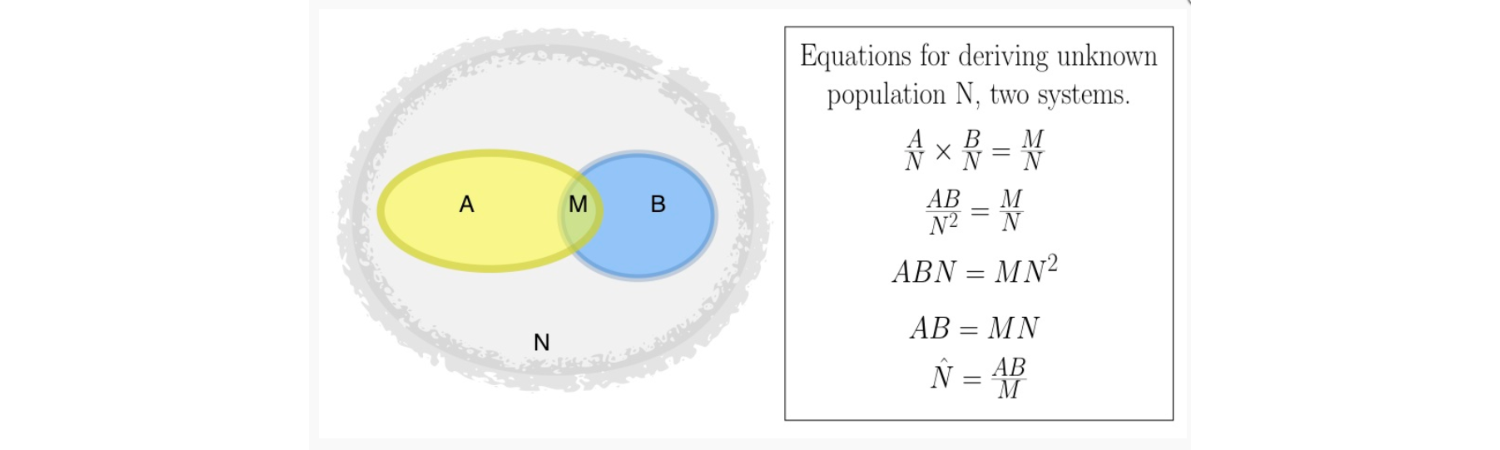
\includegraphics{Categorical-FinalProject_files/figure-latex/img.MSE-1.pdf}
\caption{Multiple System Estimation}
\end{figure}

\hypertarget{mse-assumptions}{%
\subsection{MSE Assumptions}\label{mse-assumptions}}

There are several MSE assumptions that are need for when there are two
``systems'' (lists), but not more than that. The assumptions are:

\begin{enumerate}
\def\labelenumi{\arabic{enumi}.}
\item
  \emph{Closed system}: The population of interest does not change
  during the measurement period. This means that the object of
  measurement, whether that is a population of persons in a country or a
  population of violent events that occurred in a state, is a closed
  system: the target population does not change during the period of
  measurement. This assumption is generally unproblematic for data on
  violent events, because events that occurred cannot ``un-occur''
  later.
\item
  \emph{Perfect matching (record linkage!)}: The overlap between systems
  (i.e., the group of cases recorded in more than one list) is perfectly
  identified.
\item
  \emph{Equal probability of capture}: For every data system, each
  individual has an equal probability of being captured. For example,
  every death has probability X of being recorded in list 1, every death
  has probability Y of being recorded in list 2, and so on. TThis
  assumption, the homogeneity of capture probability, is unlikely to
  hold for any type of violence data. For example, persons with fewer
  social connections may be both more likely to go missing and less
  likely to be reportedmissing; rural locations are more difficult to
  access than urban ones. Constructing two-sample estimates without
  accounting for different probabilities of capture leads to conclusions
  that may be biased.
\item
  \emph{Independence of lists}: Capture in one list does not affect
  probability of capture in another list. For example, being reported to
  one NGO does not change the probability that an individual is reported
  to another. The third assumption, independence of systems, is
  similarly difficult to meet.
\end{enumerate}

Like differences in capture probability, dependences between systems are
impossible to account for in the the two-system setting. A common
example here is the difference between governmental and non-governmental
organizations. Because different populations may have different levels
of trust in the two organizations, reporting to one type of organization
may imply that the witness is very unlikely to report to the other.

\hypertarget{overview-of-data}{%
\section{Overview of Data}\label{overview-of-data}}

\begin{table}[H]

\caption{\label{tab:data-sources}Contingency Table}
\centering
\resizebox{\linewidth}{!}{
\begin{tabular}{llrrl}
\toprule
  & Organization & Total Captures & Unique & Type\\
\midrule
d\_CCJ.n & Colombian Commision of Jurists & 214 & 48 & judicial\\
d\_EQU.n & Equitas & 22 & 0 & civil\\
d\_FON.n & Fondelibertad & 304 & 67 & security\\
d\_IMLD.n & National Institute of Forensic Medicine Disappearances & 153 & 9 & forensic\\
d\_PN0.n & Policía Nacional & 825 & 221 & security\\
\addlinespace
d\_CIN.n & CINEP & 267 & 91 & civil\\
d\_FAM.n & Families of Victims’ Organizations & 51 & 1 & civil\\
d\_FSR.n & Prosecutor General of Santa Rosa & 151 & 0 & security\\
d\_IMLM.n & Instituto Nacional de Medicina Legal & 1878 & 1219 & forensic\\
d\_VP.n & Vice Presidency Office & 501 & 284 & judicial\\
\addlinespace
d\_CCE.n & Colombia-Europe & 72 & 30 & civil\\
d\_CTI.n & Technical Investigative Body of the Prosecutor Generals Office & 36 & 0 & judicial\\
d\_FDC.n & Prosecutor General list of the Disappeared & 623 & 376 & forensic\\
d\_GAU.n & Gaula & 110 & 1 & security\\
d\_PL.n & Pais Libre & 9 & 0 & civil\\
\bottomrule
\end{tabular}}
\end{table}

\hypertarget{overall-trends}{%
\subsection{Overall Trends}\label{overall-trends}}

The following graph shows that violence has been concentrated in
\(\textcolor{red}{\text{municipality}}\). We can see that the
\emph{reported} violence (i.e.~the counts in the 15 datasets) appears to
have intensified across all municipalities in Casanare in 2003-2004 and
then dropped.

\begin{figure}
\centering
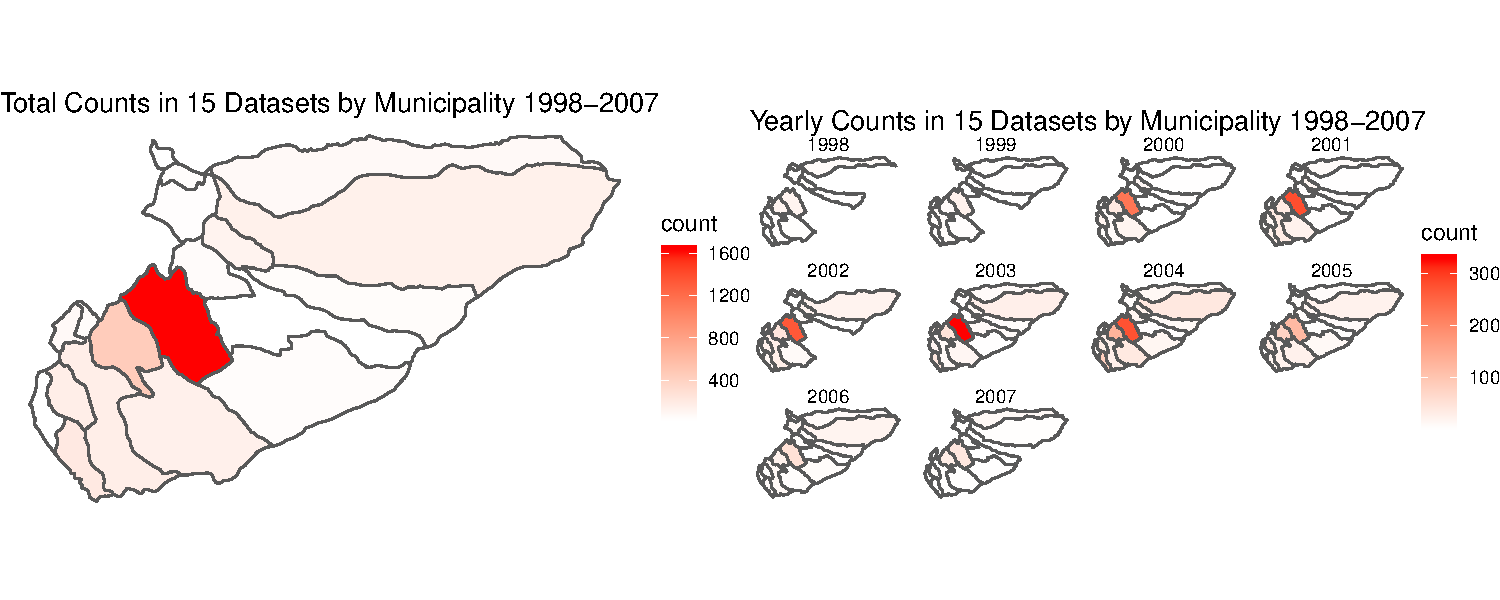
\includegraphics{Categorical-FinalProject_files/figure-latex/gisplots-1.pdf}
\caption{Overall Trends in 15 Datasets by Municipality}
\end{figure}

Looking just at the the totals of the 15 datasets and individual may
think that the violence peaked in 2003-2004 and the total of victims is
\(\textcolor{red}{\text{3000?}}\) However, just looking at the trends
amoung the totals of the 15 datasets does not give the whole picture.

\hypertarget{heterogenity-issues}{%
\subsubsection{Heterogenity Issues}\label{heterogenity-issues}}

\(\textcolor{red}{\text{AS: looking at certain year and show total, and lista, listb, listc to show diff probs}}\)

\hypertarget{different-datasets---different-stories}{%
\subsection{Different Datasets - Different
Stories}\label{different-datasets---different-stories}}

We motivate our need for a more sophisticated analysis by showing the
reporting patterns of 3 different organizations across 1998-2007. If we
relied on just one organization or even a combination of two we could
tell differnt stories regarding the violence. Relying on FAM shows a
peak in violent incidents in 2003, while reports by IMLM show a peak in
2004 . Using multiple systems estimation allows us to parse both the
reported and unreported violent in Casanare.

\begin{figure}
\centering
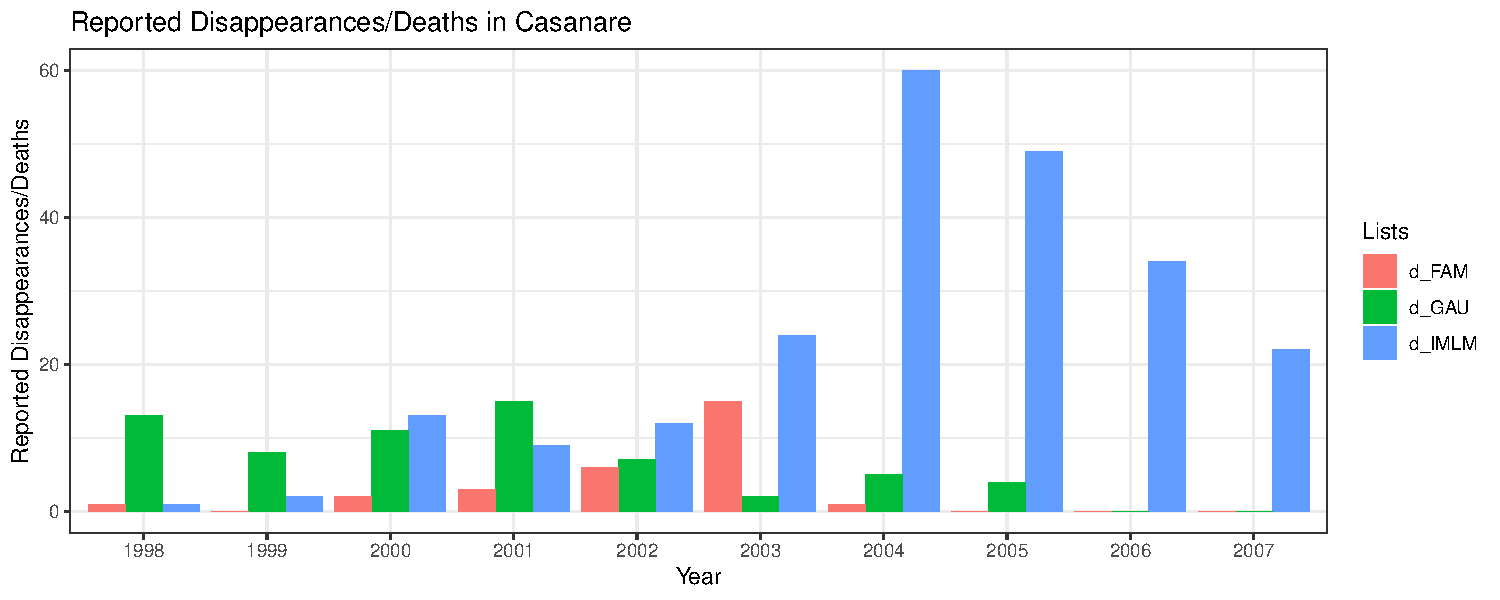
\includegraphics{Categorical-FinalProject_files/figure-latex/unnamed-chunk-1-1.pdf}
\caption{Count Trends for Three Organizations}
\end{figure}

\hypertarget{loglinear-modelling}{%
\section{Loglinear Modelling}\label{loglinear-modelling}}

In order to do our estimation, we will use loglinear modeling. We will
describe the model as if we had two datasets (for simplicity). We know
the victims ``captured'' by only dataset 1, only dataset 2, and both
datasets. However, we don't know the amount of victims that are not
captured by either list. Estimate this value allows us to estimate the
total count of victims.

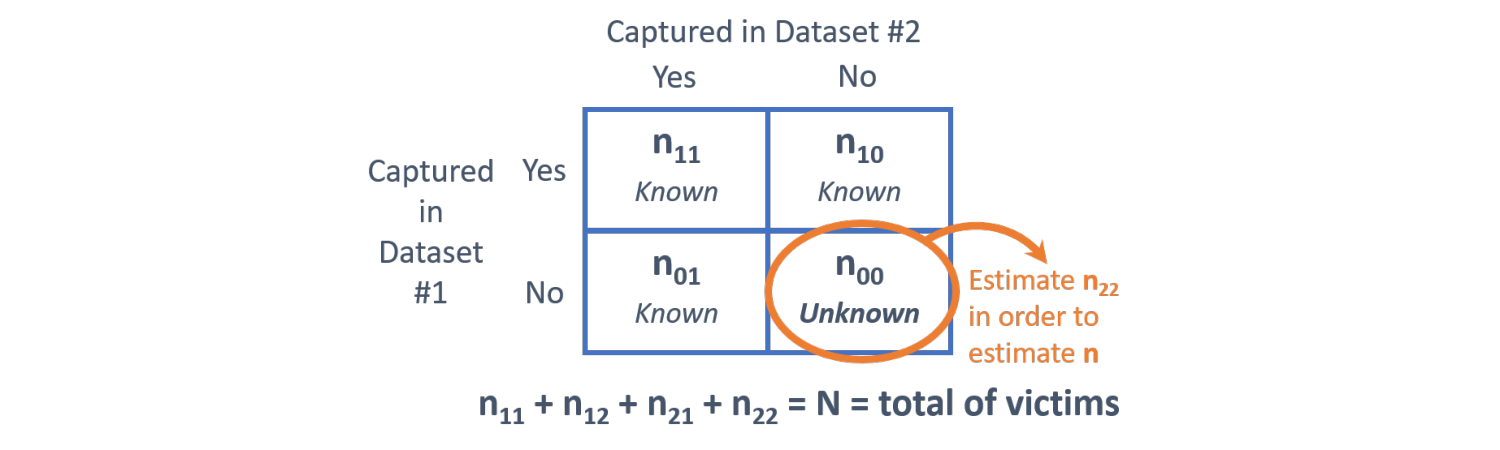
\includegraphics{Categorical-FinalProject_files/figure-latex/img.example-1.pdf}

The count of victims captured into a dataset or combindation of datasets
is \(n_{11}, n_{10}, n_{01}\), and \(n_{00}\). Each of these cells is a
count of victims captured. The subscripts denote which datasets a victim
has been captured. The subscripts denotes if the victim has been
captured (1), or not been captured by a certain data set. For
\(n_{ij}\), \(i\) is for dataset \#1 and \(j\) is dataset \#2.

Our estimates are primarily based on Poisson regression. Poisson
regression treaets these cell counts - not the underlying individual
cases data

\hypertarget{estimating-the-total-count-of-victims}{%
\subsection{Estimating the Total Count of
Victims}\label{estimating-the-total-count-of-victims}}

We are interested in estimating \(n_{00}\), which also allows us to
estimate the total number of victims.\\
The (log of the) expected cell count \(n_{00}\) is a function of the
other observed cell counts, as shown in the equation below.

\[
\log(n_{00}) = \alpha 
+ \beta_1 \cdot \mathbbm{1}(x\in n_{10}) 
+ \beta_2 \cdot \mathbbm{1}(x\in n_{01}) 
\]

This is the saturated form of the log-linear models introduced in
Bishop, Fienberg and Holland (1975). To quote from Agresti, ``the
saturated GLM has a separate parameter for each observation. It gives a
perfect fit. This sounds good, but it is not a helpful model. It does
not smooth the data or have the advantages that a simpler model has,
such as parsimony. Nonetheless, it serves as a baseline for other
models, such as for checking model fit.''

When estimation of the total ``population'' of missing people in
Casanare is the goal (as it typically is with multiple-systems
estimation), the key value here is the intercept \(\alpha\). To estimate
\(\log(n_{00}\)), all the other values in the model are zero, as the
indicator functions for \(n_{ij}\) for zero. Therefore the only term
that contributes to the estimate of \(\log(n_{00}\)) is \(\alpha\). The
value of \(n_{00}\) is therefore the exponentiated value of \(a\), that
is, \(\exp(\alpha)\). The total number of cases, \(N\), is the sum of
the observed cases plus \(\exp(\alpha)\).

\[
\begin{aligned}
\log(n_{00}) &= \alpha 
\underbrace{
+ \beta_1 \cdot  \mathbbm{1}(x\in n_{10}) 
+ \beta_2 \cdot \mathbbm{1}(x\in n_{01}) 
}_{\text{each }=0}
\\[.5ex]
\log(n_{00}) & = \alpha 
\\[.5ex]
\hat{n}_{00} & = \exp \left\{ \hat{\alpha} \right\}
\\[3ex]
\hat{N} &= n_{11} + n_{10} + n_{01} + \hat{n}_{00}
\end{aligned}
\]

As with any regression and data mining model, we want to avoid
overfitting. There is a tradeoff we need to balance between ``goodness
of fit'', and simple (parsimonious) models.

We need to find the best model in order to get an accurate estimate of
\(\alpha\). Thus, we should determine whether the full (saturated) model
above, which assumes that all three two-way interactions between
datasets are important, is actually necessary. There is one simpler
models that assume the two-way interaction.

\[
\log(n_{00}) = \alpha 
+ \beta_1 \cdot \mathbbm{1}(x\in n_{10}) 
+ \beta_2 \cdot \mathbbm{1}(x\in n_{01}) 
+ \beta_{12} \cdot \mathbbm{1}(x \in n_{11})
\]

In this case, we can clearly write out the possible model. During model
selection, we estimate these models and choose the model that minimizes
the Bayesian Information Criterion (BIC), a test that weighs goodness of
fit against degrees of freedom.

\hypertarget{challenges-with-loglinear-models}{%
\subsection{Challenges with Loglinear
models}\label{challenges-with-loglinear-models}}

\begin{enumerate}
\def\labelenumi{\arabic{enumi}.}
\tightlist
\item
  \textbf{Interpretation:} The inclusion of so many variables in
  loglinear models often makes interpretation very difficult.\\
\item
  \textbf{Independence Assumption:} The frequency in each cell is
  independent of frequencies in all other cells, which is not
  necessarily the case here. We attempt to model this.\\
\item
  \textbf{Sample Size Requirement:} With loglinear models, you need to
  have at least 5 times the number of cases as cells in your data. If
  you do not have the required amount of cases, then you need to
  increase the sample size or eliminate one or more of the variables.
\end{enumerate}

\hypertarget{choosing-our-systems}{%
\subsection{Choosing our ``Systems''}\label{choosing-our-systems}}

Our dataset encompasses 15 datasets, far too many to model with a
loglinear model. We collapse these 15 datasets into 4 systems
(i.e.~groups) based on the type of organization that produced the
dataset.

\begin{table}[H]

\caption{\label{tab:adding-systems}Example of Information from Systems}
\centering
\begin{tabular}{rrrrr}
\toprule
security\_ind & forensic\_ind & judicial\_ind & civil\_ind & Freq\\
\midrule
0 & 0 & 0 & 1 & 5\\
0 & 0 & 1 & 0 & 1\\
0 & 0 & 1 & 0 & 1\\
1 & 0 & 0 & 0 & 1\\
1 & 0 & 1 & 0 & 1\\
\addlinespace
0 & 0 & 1 & 1 & 1\\
\bottomrule
\end{tabular}
\end{table}

\begin{figure}
\centering
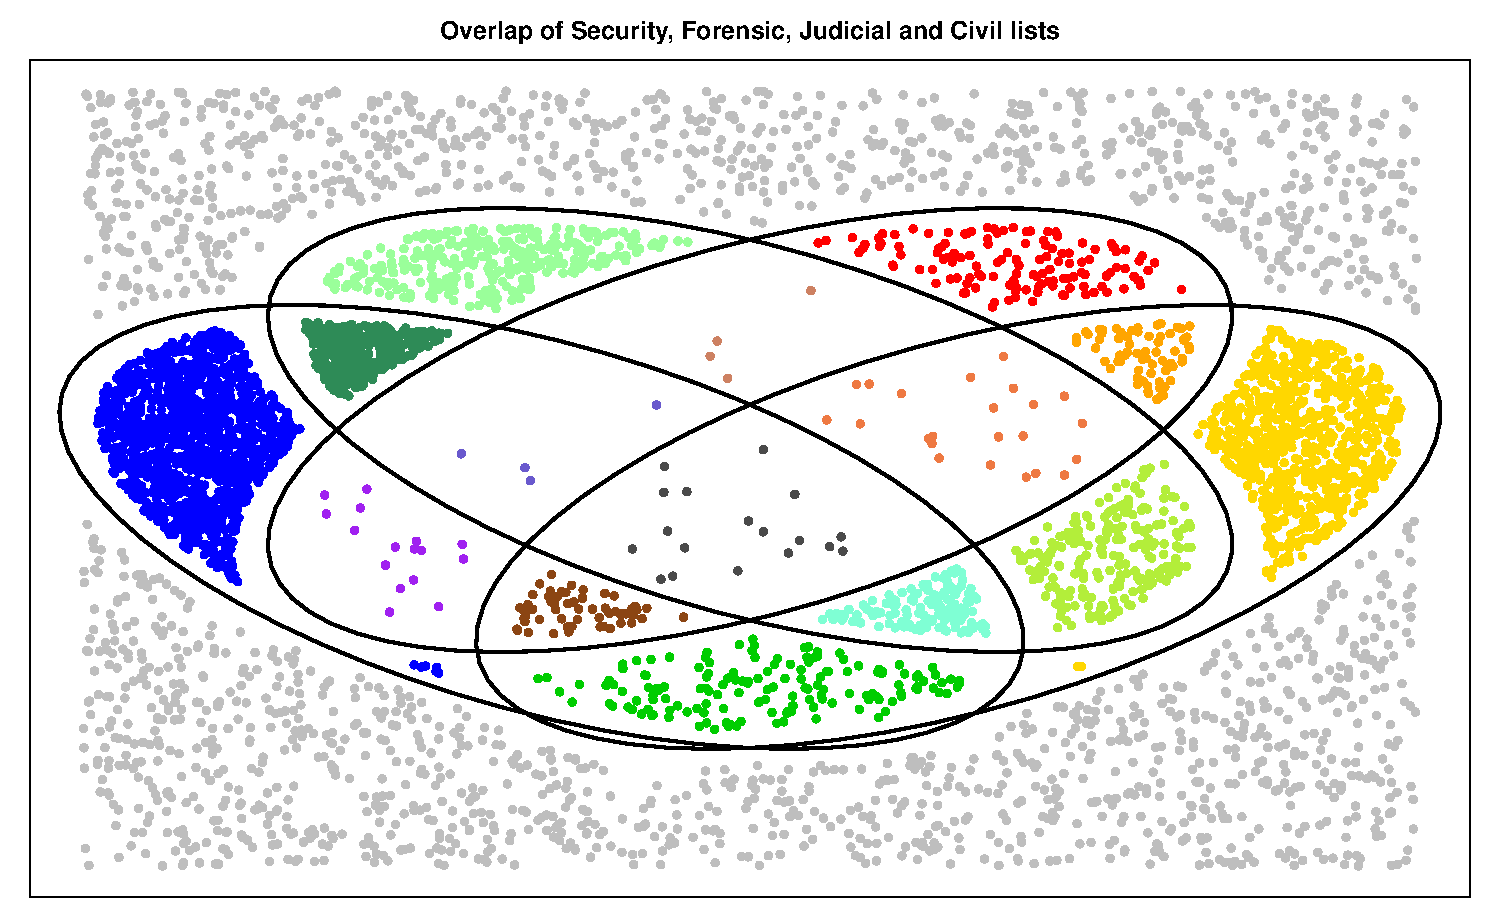
\includegraphics{Categorical-FinalProject_files/figure-latex/systems.venndiagram-1.pdf}
\caption{Estimated Venn Diagram of Systems}
\end{figure}

In the above Venn Diagram, the colored dots represent a specific victim.
We are trying to estimate the victims that are not caputred in one of th
lists (shown by the graph dots). We can see there is not a lot of
overlap, which suggests there may be lack of heterogenity capture
probability (i.e.~the probability of a victim captured differs from list
to list). In addition, this implies that there is likely a much larger
population of victims than counted in the 15 datasets.

\hypertarget{model-definitions}{%
\subsection{Model Definitions}\label{model-definitions}}

\hypertarget{types-of-models}{%
\subsubsection{Types of Models}\label{types-of-models}}

Models will be donoted by \(M\), and the subscripts will denote the type
of model.

\begin{itemize}
\tightlist
\item
  \(M_0\): The \(M_0\) model is the simplest possible multiple source
  capture recapture model. It assumes that there is no heterogeneity and
  that all lists (civil, security, judicial, etc) have the same
  probability of capturing individuals. We know that this is not the
  case here.
\item
  \(M_t\): This model relaxes the \(M_0\) model to allow for lists to
  have different capture rates.
\item
  \(M_h\): This model relaxes the \(M_0\) model to allow for individual
  capture heterogeneity.
\item
  \(M_{th}\): This model allows for both list heterogeneity and capture
  events having different rates.
\end{itemize}

\hypertarget{types-of-heterogeniety}{%
\subsubsection{Types of Heterogeniety}\label{types-of-heterogeniety}}

When heterogeneity in capture probability is present (i.e.~the
probability of a list capturing a victims differs), there are different
forms that this heterogeneity can take.

\begin{itemize}
\tightlist
\item
  Normal: The log odds of capture follows a Normal distribution.
\item
  Darroch: The log odds of capture among those who were not captured
  follows a Normal distribution.
\item
  Poisson: The log odds of capture among those who were not captured
  follows a Poisson distribution.
\item
  Gamma: The log odds of capture among those who were not captured
  follows a Gamma distribution.
\end{itemize}

\hypertarget{non-hierarchical-models}{%
\subsection{Non-Hierarchical Models}\label{non-hierarchical-models}}

After collapsing the 15 lists into four systems, we fit several
loglinear models. We see that the best fits clearly take into account
both system and individual heterogeneity. We therefore choose the
\(M_{th}\) model with the log odds of capture among those who were not
captured follows a Gamma distribution. We see that the \(M_0\) model
demonstrates a clear lack of fit, which we would expect for this data.
The models listed below are \emph{not} hierchachal in nature.

We will need the hierchachal structure to perform model selection. It's
important to note that a model is not chosen if it bears no resemblance
to the observed data. The choice of a preferred model is typically based
on a formal comparison of goodness-of-fit statistics associated with
models that are related hierarchically (models containing higher order
terms also implicitly include all lower order terms). Ultimately, the
preferred model should distinguish between the pattern of the variables
in the data and sampling variability, thus providing an intuitive
interpretation.

The ``number of captured units'' is the number of observed elements, in
this example, the number of people documented as missing/killed, we
usually call this \(N_c\) (\(N\) for overall total, and \(c\) denoting
caputred. The ``abundance'' column shows the estimate of \(\hat{N}\),
the total population including the observed and the estimated unobserved
deaths. The AIC and BIC columns show the ``information coefficients''
which balance the goodness of fit (shown in the ``deviance'' column)
with the information used to estimate the model (degrees of freedom
indicate this). Model selection often occurs based on the smallest AIC
and BIC values, however this can only be done with hierchical models
which is not the case here.

\begin{table}[H]

\caption{\label{tab:NOT-HIERCH-models}Summary of Models (Non-hierarchical models)}
\centering
\begin{tabular}{lrrrrrrr}
\toprule
  & abundance & stderr & deviance & df & AIC & BIC & infoFit\\
\midrule
M0 & 5604.929 & 100.60691 & 2279.4707 & 13 & 2376.7355 & 2389.0571 & 0\\
Mt & 5232.814 & 87.30936 & 529.8227 & 10 & 633.0875 & 663.8915 & 0\\
Mh Chao (LB) & 5970.687 & 139.89294 & 2253.9791 & 12 & 2353.2439 & 2371.7263 & 0\\
Mh Poisson2 & 6147.489 & 188.43134 & 2262.1217 & 12 & 2361.3865 & 2379.8689 & 0\\
Mh Darroch & 6866.486 & 367.88961 & 2257.9368 & 12 & 2357.2016 & 2375.6840 & 0\\
\addlinespace
Mh Gamma3.5 & 7725.102 & 634.44312 & 2256.6358 & 12 & 2355.9007 & 2374.3831 & 0\\
Mth Chao (LB) & 5665.285 & 125.06924 & 473.7645 & 8 & 581.0293 & 624.1550 & 0\\
Mth Poisson2 & 6035.010 & 181.67803 & 482.2671 & 9 & 587.5319 & 624.4967 & 0\\
Mth Darroch & 7204.688 & 411.30447 & 476.0572 & 9 & 581.3221 & 618.2869 & 0\\
Mth Gamma3.5 & 8782.672 & 810.69350 & 474.7154 & 9 & 579.9802 & 616.9450 & 0\\
\addlinespace
Mb & 4228.193 & 64.66437 & 2107.1837 & 12 & 2206.4485 & 2224.9309 & 0\\
Mbh & 3643.007 & 47.70713 & 1618.9871 & 11 & 1720.2520 & 1744.8952 & 0\\
\bottomrule
\end{tabular}
\end{table}

Each model controls for a subset of all the possible interactions among
the models. In the context of MSE, the two- and three-way interactions
estimate (and to some extent, control for) associations in the
probabilities of capture between (and among) the lists. For example, is
a certain person more likely to be seen on one list, and also more
likely to be seen on a second list? If associations like this are
present (and they usually are), they can bias the estimate.

\begin{figure}
\centering
\includegraphics{Categorical-FinalProject_files/figure-latex/NOT-HIERCH-models-boxplot-1.pdf}
\caption{Boxplot of Residuals for Models}
\end{figure}

These boxplots of residuals offer a general assesment of model fit. The
light dotted line represents zero, and ideally you want the residuals
centered around zero. We see that there is significantly less variation
in the \(M_{th}\) Models. These models account for list heterogenity
(probability of capture for a specific victim varies from list to list)
and individual heterogenity (probability of capture for a specific list
varies from victim to victim). Models that account for heterogenity
offer less variation but also do not have residuals centered at zero.

\hypertarget{specific-model-results}{%
\subsection{Specific Model Results}\label{specific-model-results}}

\begin{figure}
\centering
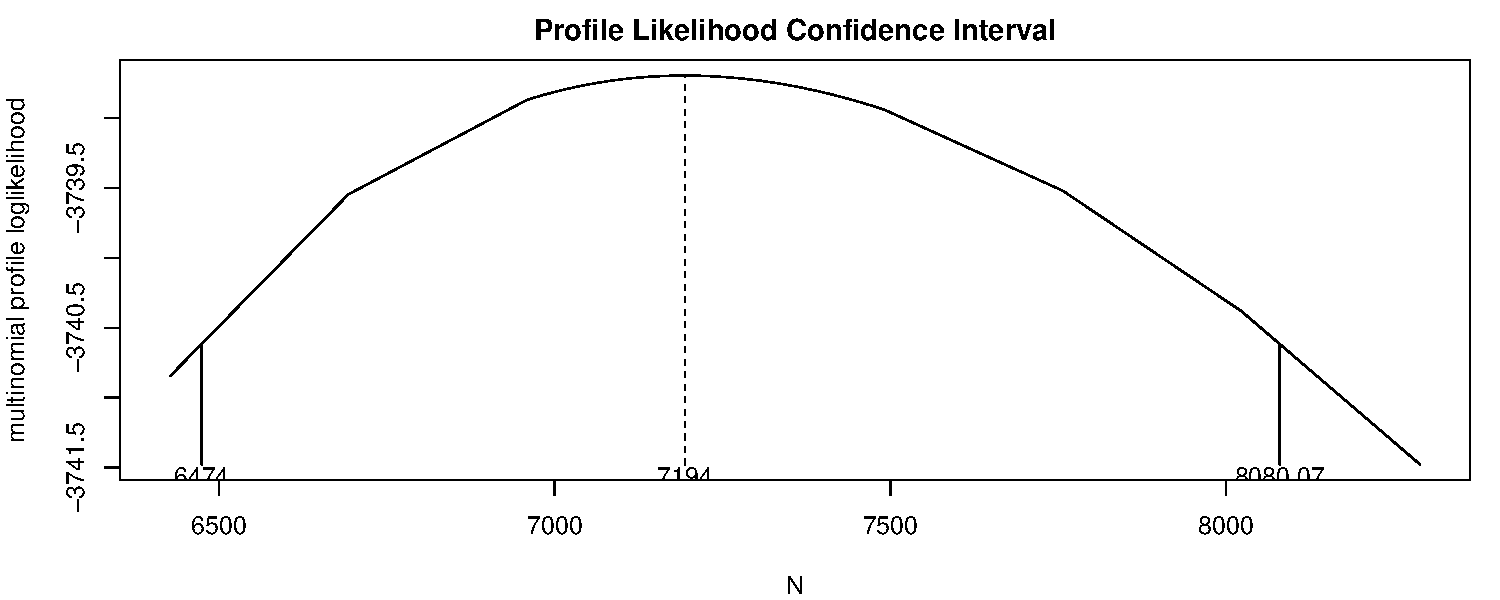
\includegraphics{Categorical-FinalProject_files/figure-latex/modelProfileLike-1.pdf}
\caption{Profile Likelihood of Specific Model}
\end{figure}

\begin{table}[H]

\caption{\label{tab:modelProfileLikeCI}Confidence Interval of Specific Model}
\centering
\begin{tabular}{lrrr}
\toprule
  & abundance & InfCL & SupCL\\
\midrule
Mth Darroch & 7194 & 6474 & 8080.07\\
\bottomrule
\end{tabular}
\end{table}

\hypertarget{capture-recapture}{%
\subsection{Capture Recapture}\label{capture-recapture}}

We display some basic capture-recapture frequency statistics to explore
capture patterns. It displays, for \(i= 1,...t\), the number of people
captured \(i\) times (\(f_i\)), the number of people captured for the
first time on occasion \(i\) (\(u_i\)), the number of units capturedfor
the last time on occasion \(i\) (\(v_i\)) and the number of units
captured on occasion \(i\) (\(n_i\)). If the \(n_i\) statistics vary
among capture occasions, there is a temporal effect-- which we clearly
see here. We would expect the top panel of the plot to be linear, while
the bottom panel should be concave down or exhibit no pattern for
capture patterns that are best fit with \(M_{th}\) models.

\begin{verbatim}
## 
## Number of captured units: 3501 
##  
## Frequency statistics:
##        fi    ui    vi    ni  
## i = 1  2392  1128   317  1128
## i = 2   866  1455  1640  2028
## i = 3   225   785  1216  1387
## i = 4    18   133   328   328
## fi: number of units captured i times
## ui: number of units captured for the first time on occasion i
## vi: number of units captured for the last time on occasion i
## ni: number of units captured on occasion i
\end{verbatim}

\begin{figure}
\centering
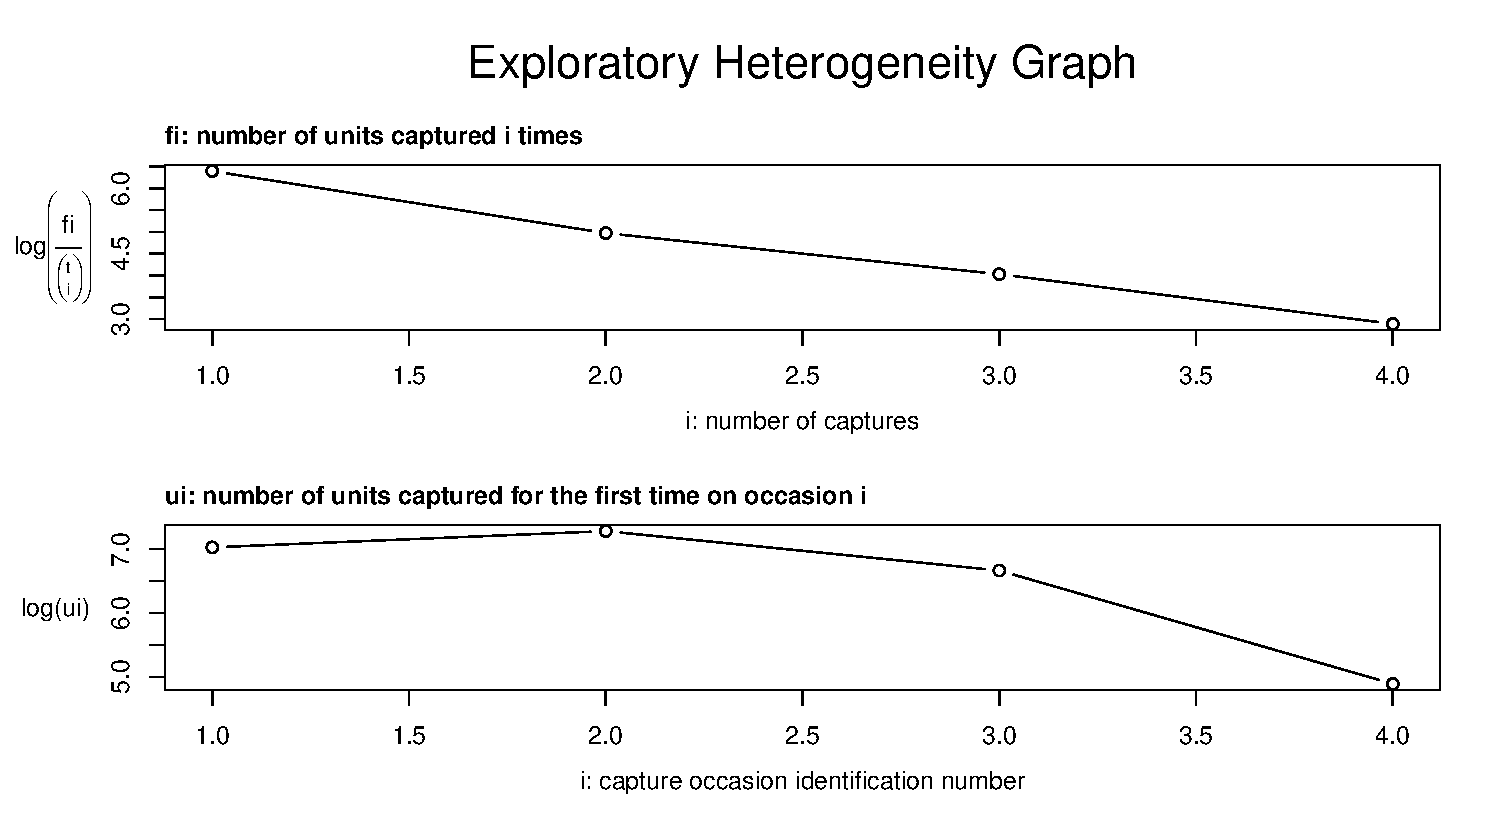
\includegraphics{Categorical-FinalProject_files/figure-latex/descriptive-stats-1.pdf}
\caption{Capture-Recapture Frequency Statistics}
\end{figure}

\[\log\left(\frac{f_i}{{t \choose i}}\right) = \log \left(\frac{N \times P(i \text{ captures})}{{t \choose i}}\right) = \log(N(1-p)^{t-i} p^i = \log(N(1-p)^t) + i\log\left(\frac{p}{1-p}\right)\]

\hypertarget{hierarchical-models-choosing-a-model}{%
\subsection{Hierarchical Models: Choosing a
Model}\label{hierarchical-models-choosing-a-model}}

The iterative proportional fitting process generates maximum likelihood
estimates of the expected cell frequencies for a hierarchical model. In
short, preliminary estimates of the expected cell frequencies are
successfully adjusted to fit each of the marginal sub-tables specified
in the model.

\(\textcolor{red}{\text{AS: wants to rewrite}}\)\\
For example, in the model \(list_1\), \(list_{12}\), \(list_{123}\), the
initial estimates are adjusted to fit \(list_{12}\) then \(list_{23}\)
and finally to equal the \(list_{123}\), observed frequencies. The
previous adjustments become distorted with each new fit, so the process
starts over again with the most recent cell estimate. This process
continues until an arbitrarily small difference exists between the
current and previous estimates.

We fit hierchachal models, restricting to second-order (no three-way
interactions) for sake of interpretation.The best model according to the
BIC criteria, is below: estimates a total for missing/disappeared people
as \(8607\), which is similar to the \(8782\) than that of the
non-hierch., interactionless, model.

The below describes three possible models. The \(\log(\hat{N})\) is
based on the grand mean \(\mu\) and effects based on our 4 systems
(which are represented by \(\lambda\)). The subscripts of \(\lambda\)
denote whether the effect is coming from a single system or the overlap
between two systems (note we did not look at models that more than
two-way interactions).

\[
\begin{aligned}
\text{Top Model:}\quad & \log(\hat{N}) = \mu + \lambda_{12} + \lambda_{13} + \lambda_{14} + \lambda_{23} + \lambda_{24} + \lambda_{34}
\\
\text{Example of Middle Model:}\quad & \log(\hat{N}) = \mu +  \lambda_{13} + \lambda_{14} + \lambda_{24}
\\
\text{Bottom Model:}\quad & \log(\hat{N}) = \mu + \lambda_1 + \lambda_2 + \lambda_3 + \lambda_4 
\end{aligned} 
\]

\begin{table}[H]

\caption{\label{tab:hierch-models}'Top' Five, 'Middle' Five, and 'Bottom' Five Models (Hierarchical models)}
\centering
\resizebox{\linewidth}{!}{
\begin{tabular}{lrrrrrrrr}
\toprule
  & abundance & stderr & bias & deviance & df & AIC & BIC & infoFit\\
\midrule
12,13,14,23,24,34 & 8817.112 & 1515.7607 & 237.8220039 & 72.33182 & 3 & 189.5966 & 263.5263 & 0\\
12,13,14,23,24 & 5076.249 & 168.5601 & 9.6710160 & 93.42304 & 4 & 208.6879 & 276.4567 & 0\\
12,13,14,23,34 & 7308.085 & 455.7503 & 36.3107669 & 73.99807 & 4 & 189.2629 & 257.0317 & 0\\
12,13,14,24,34 & 8695.570 & 493.7868 & 32.6905220 & 72.33923 & 4 & 187.6040 & 255.3729 & 0\\
12,13,23,24,34 & 9267.442 & 876.2745 & 91.6873828 & 72.44539 & 4 & 187.7102 & 255.4791 & 0\\
\addlinespace
12,24,34 & 6990.394 & 275.9882 & 8.1501334 & 251.01919 & 6 & 362.2840 & 417.7312 & 0\\
13,14,23 & 5388.545 & 160.4725 & 6.9759022 & 180.47969 & 6 & 291.7445 & 347.1917 & 0\\
13,14,24 & 6408.681 & 225.7425 & 8.3355958 & 397.52853 & 6 & 508.7934 & 564.2406 & 0\\
13,23,24 & 5052.802 & 130.3749 & 3.2161351 & 209.76658 & 6 & 321.0314 & 376.4786 & 0\\
13,23,34 & 5178.863 & 140.5477 & 3.1073571 & 223.51518 & 6 & 334.7800 & 390.2272 & 0\\
\addlinespace
14,2,3 & 6349.780 & 217.6530 & 6.4628534 & 444.04882 & 8 & 551.3136 & 594.4393 & 0\\
23,1,4 & 5076.432 & 127.2073 & 1.1770391 & 278.46874 & 8 & 385.7336 & 428.8592 & 0\\
24,1,3 & 6089.940 & 188.3562 & 2.6692553 & 450.63028 & 8 & 557.8951 & 601.0207 & 0\\
34,1,2 & 5903.270 & 172.5871 & 1.4531676 & 404.10047 & 8 & 511.3653 & 554.4909 & 0\\
1,2,3,4 & 6035.010 & 181.6780 & 0.7620688 & 482.26705 & 9 & 587.5319 & 624.4967 & 0\\
\bottomrule
\end{tabular}}
\end{table}

We also plot the BIC values for different models and their accompanying
estimates of \(\hat{N}\).

Note that these the hierch. models have different estimates ,ranging
from 5231 to 8607, all within very similar BIC values Which one should
we use?

\begin{figure}
\centering
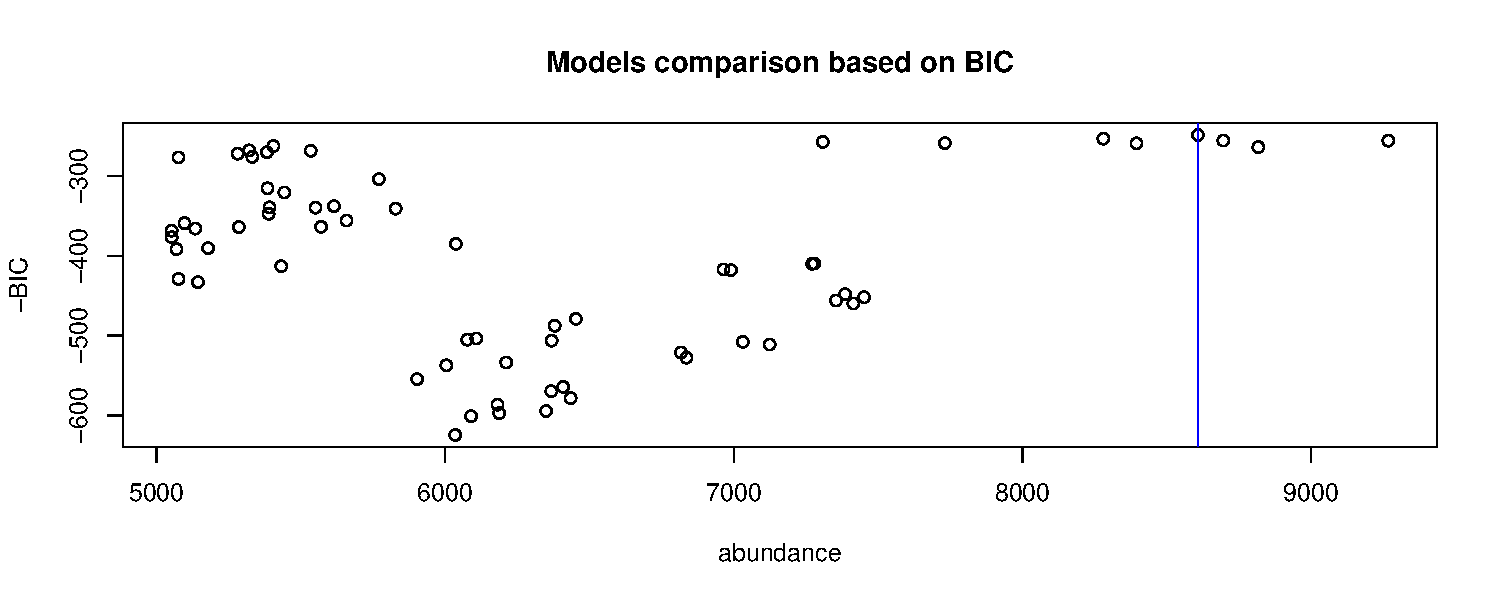
\includegraphics{Categorical-FinalProject_files/figure-latex/hierch-modelsBIC-1.pdf}
\caption{Hiercharical Models BIC Plot}
\end{figure}

This is the fundamental problem of the frequentist approach. We could
just pick the ``best'' model, i.e., the one with the lowest BIC.
Unfortunately, just picking one model ignores the error that we
introduce by the selection itself. It also forces us to decide which
dependencies among the systems we will control for, forcing us to decide
which dependencies will not be included in the model.

\hypertarget{goodness-of-fit}{%
\section{Goodness of Fit}\label{goodness-of-fit}}

\(\textcolor{red}{\text{AS}}\)

I will describe here how likelihood ratio test is better for model
comparison than Pearson's Chi-square??

\hypertarget{conclusions}{%
\section{Conclusions}\label{conclusions}}

\(\textcolor{red}{\text{MB}}\)

\begin{itemize}
\tightlist
\item
  total under 15 datasets 3000 (? check this number )
\item
  Lots of uncertaintiy (not even sure our data meets requirements for
  modeling)
\item
  ``valid'' estimates can range from 5000 - 9000 (could be used for
  different political stories)
\end{itemize}


\end{document}
